\section[组合编码和伪距观测]{组合编码和伪距观测\\Combined Code and Phase Observations}
GPS observations are characterized by a multitude of data collected at short time intervals varying from 1 s to say 30s. The data are processed by least squares or the filtering techniques described in this chapter. This happens in real time or in post processing mode.Computational methods that focus on high accuracy require longer times. Other methods concentrate on short processing time or real time availability.

Today the best geodetic receivers deliver dual frequency P code and phase observations.We shall restrict ourselves to the latest methods for processing data observed with static antennas. The accuracy is greatest with post processing.

A popular procedure for processing GPS observations uses double differences. Such double differences are quite insensitive to shared changes of position of the two receivers,but they are very sensitive to changes of one receiver relative to the other. Therefore,double differences resemble classical distance and direction observations.

In order to separate geometry (the baseline between two receivers) from ambiguities in the cycle count, we want a lot of data. With no a priori knowledge, it is difficult within a short period of time to distinguish the baseline from the ambiguities. But as time goes by,hopefully only one baseline fits the double differenced observations. The more satellites that are observed, the faster the baseline can be dcetermined. As soon as the baseline is uniquely determined within a fraction of a cycle (a wavelength), an ambiguity can be fixed to its integer value. This is the key to optimal use of double differenced observations.

Usually the ambiguities and the baseline vector are estimated by least squares. That is, the best estimates of the ambiguities and the baseline are those values which minimize the squared sum of residuals. Ambiguities are often treated as reals! As the systematic errors are eliminated , the ambiguities tend to their integer values. The classical case involves short baselines for which ambiguities are safely determined.

\begin{figure}
	\centering
	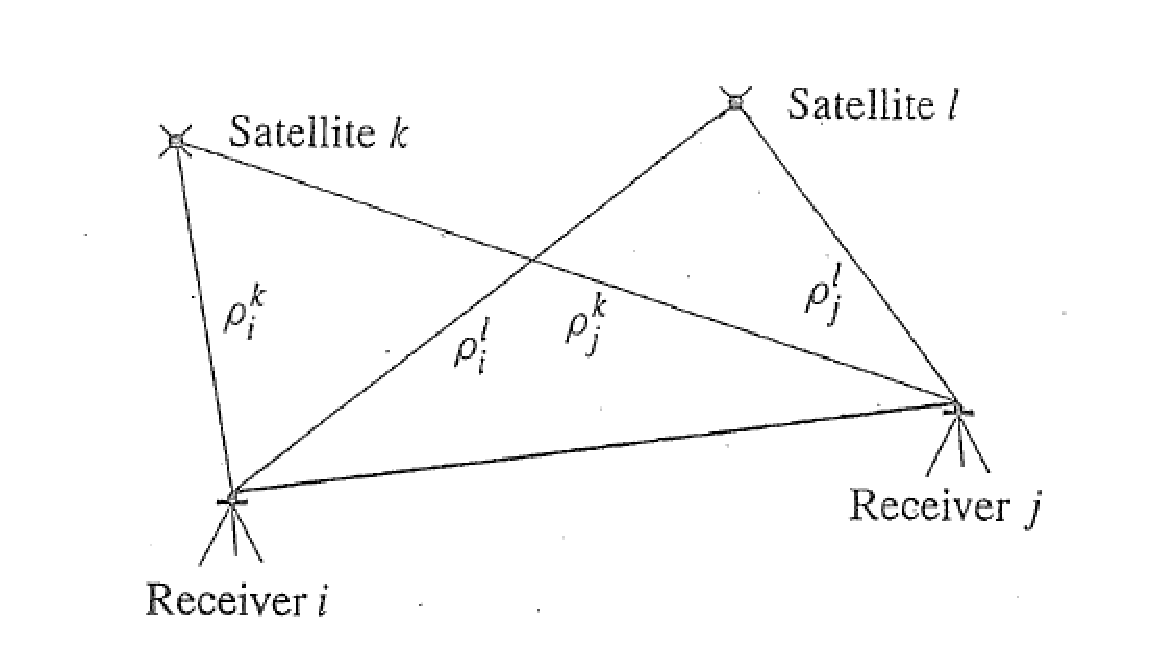
\includegraphics[width=0.4\linewidth]{TeX_files/Part03/chapter10/image/9-2}
	\caption{Double difference $\rho_{i}^{k}-\rho_{i}^{l}-\rho_{j}^{k}+\rho_{j}^{l}$. Two receivers observe pseudoranges from two satellites at the same time.}
	\label{fig:9-2}
\end{figure}

For reference, we shall use the terminology already introduced by Yang \& Goad \& Schaffrin (1994). The ideal pseudorange $\rho^{*}$ is a combination of all frequency independent clock-based terms:

\begin{equation}
\rho_{i}^{*k}=\rho_{i}^{k}(t,t-\tau_{i}^{k})+T_{i}^{k}+c(dt_{i}(t)-dt^{k}(t-\tau_{i}^{k}))
\end{equation}

If the ionospheric effect $I_{i}^{k}$ were zero ,$\rho^{*}$ would be identical to the pseudorange $\rho$. The term $T_{i}^{k}$ denotes the tropospheric delay. The terms in parentheses cancel when we use double differenced observations, because these are clock errors.

A phase observation $\Phi_{i}^{k}(t)$ is the difference in phase from a signal generated at the same frequency as pseudorange. The basic equation is��

\begin{equation}
\Phi_{i}^{k}(t)=\rho_{i}^{k}-I_{i}^{k}+T_{i}^{k}+c(dt_{i}(t)-dt^{k}(t-\tau_{i}^{k}))+\lambda(\varphi_{i}(t_{0})-\varphi^{k}(t_{0}))+\lambda N_{i}^{k}-\epsilon_{i}^{k}
\end{equation}

The new terms are the ambiguities $N_{i}^{k}$ and receiver i , and the non-zero initial phases $\varphi^{k}(t_{0})$ and $\varphi_{i}(t_{0})$. Again we introduce the ideal pseudorange given above:

\begin{equation}
\Phi_{i}^{k}(t)=\rho_{i}^{*k}+\lambda N_{i}^{*k}
\end{equation}

where $N_{i}^{*k}=N_{i}^{k}+\varphi_{i}(t_{0})-\varphi^{k}(t_{0})$. For double differences the two $\varphi$ terms and the two dt terms cancel. This means that in case of double differences $N_{ij}^{*kl}=N_{ij}^{kl}$. This applies below in (10.6) and (10.7).

We shall demonstrate in detail how to make double differences of the observations.The original observation is a (one-way) difference between a receiver and a satellite. To eliminate the satellite clock error we make differences between two receivers and one satellite.Finally the double difference between two receivers and two satellites also eliminates receiver clock errors. The receivers are i and j , the satellites are k and l:

\begin{equation}
On L1: P_{1,ij}^{kl}=\rho_{i}^{k}-\rho_{i}^{l}-\rho_{j}^{k}+\rho_{j}^{l}+I_{ij}^{kl}+T_{ij}^{kl}-e_{1,ij}^{kl}
\end{equation}

\begin{equation}
On L2: P_{2,ij}^{kl}=\rho_{i}^{k}-\rho_{i}^{l}-\rho_{j}^{k}+\rho_{j}^{l}+(f_{1}/f_{2})^{2}I_{ij}^{kl}+T_{ij}^{kl}-e_{2,ij}^{kl}
\end{equation}

Explicitly $T_{ij}^{kl}=(T_{i}^{k}-T_{i}^{l})-(T_{j}^{k}-T_{j}^{l})$��and similarly for $I_{ij}^{kl}$, $N_{ij}^{kl}$, and $\epsilon_{ij}^{kl}$. Subscripts 1 and 2 refer to L1 and L2 signals with frequencies $f_{1}$ and $f_{2}$. In order to emphasize the influence of geometry we have left the $\rho$ terms uncombined; they are also double differences,so are the phase observations:

\begin{equation}
\Phi_{1,ij}^{kl}=\rho_{i}^{k}-\rho_{i}^{l}-\rho_{j}^{k}+\rho_{j}^{l}-I_{ij}^{kl}+T_{ij}^{kl}+\lambda_{1} N_{1,ij}^{kl}-\epsilon_{1,ij}^{kl}
\end{equation}

\begin{equation} \Phi_{2,ij}^{kl}=\rho_{i}^{k}-\rho_{i}^{l}-\rho_{j}^{k}+\rho_{j}^{l}-(f_{1}/f_{2})^{2}I_{ij}^{kl}+T_{ij}^{kl}+\lambda_{2} N_{2,ij}^{kl}-\epsilon_{2,ij}^{kl}
\end{equation}

The ionospheric delay is frequency-dependent (dispersive ); $\alpha=(f_{1}/f_{2})^{2}$ multiplies this delay I for the L2 observations. Actually, we have $f_{1}/f_{2}$ = 154/120 = 1.283333....The group delay is connected to the distances P while the phase advance is connected to the phase observations $\Phi$. Thus, we see a reversed sign for I in (10.6) and (10.7). All observational errors are included in the $e_{ij}^{kl}$ and $\epsilon_{ij}^{kl}$ terms.

The rest of this chapter deals exclusively with double differenced observations. We also omit the subscripts and superscripts related to the receivers and satellites, since there are exactly two of each:

\begin{equation}
\begin{split}
P_{1}=\rho^{*}+I-e_{1}\\
\Phi_{1}=\rho^{*}-I+\lambda_{1}N_{1}-\epsilon_{1}\\
P_{2}=\rho^{*}+\alpha I-e_{2}\\
\Phi_{2}=\rho^{*}-\alpha I+\lambda_{2}N_{2}-\epsilon_{2}
\end{split}
\end{equation}

equation (10.8) is transformed by Yang \& Goad \& Schaffrin (1994) into the elegant matrix equation

\begin{equation}
\begin{bmatrix}
P_{1}\\
\Phi_{1}\\
P_{2}\\
\Phi_{2}\\
\end{bmatrix}
=\begin{bmatrix}
1 & 1 & 0 & 0\\
1 & -1 & \lambda_{1} & 0\\
1 & \alpha & 0 & 0\\
1 & -\alpha & 0 & \lambda_{2}\\
\end{bmatrix}
\begin{bmatrix}
\rho_{*}\\
I\\
N_{1}\\
N_{2}\\
\end{bmatrix}
-
\begin{bmatrix}
e_{1}\\
\epsilon_{1}\\
e_{2}\\
\epsilon_{2}\\
\end{bmatrix}
\end{equation}

When all e and $\epsilon$ values are set to zero, we can solve the four equations to find the four unknowns. This determines the ideal pseudorange $\rho_{*}$, the instantaneous ionospheric delay I ,and the ambiguities $N_{1}$ and $N_{2}$. The inverse coefficient matrix that solves the equation is

\begin{equation}
\begin{bmatrix}
\frac{\alpha}{\alpha-1}&0&-\frac{1}{\alpha-1}&0\\
-\frac{1}{\alpha-1}&0&\frac{1}{\alpha-1}&0\\
-\frac{\alpha+1}{\lambda_{1}(\alpha-1)}&\frac{1}{\lambda_{1}}&\frac{2}{\lambda_{1}(\alpha-1)}&0\\
-\frac{2\alpha}{\lambda_{2}(\alpha-1)}&0&\frac{\alpha+1}{\lambda_{2}(\alpha-1)}&\frac{1}{\lambda_{2}}\\
\end{bmatrix}
\end{equation}

with eigenvalues (-0.646, 0.670, 4.095, 18.768).

\subsection{easy8}

Any professional GPS software needs to check for cycle slips and resets of the receiver clock (Figure 10.3). The reset in the receiver clock is typically one millisecond , and it influences the pseudoranges alone, while cycle slips spoil the carrier phase observations.

\begin{figure}
	\centering
	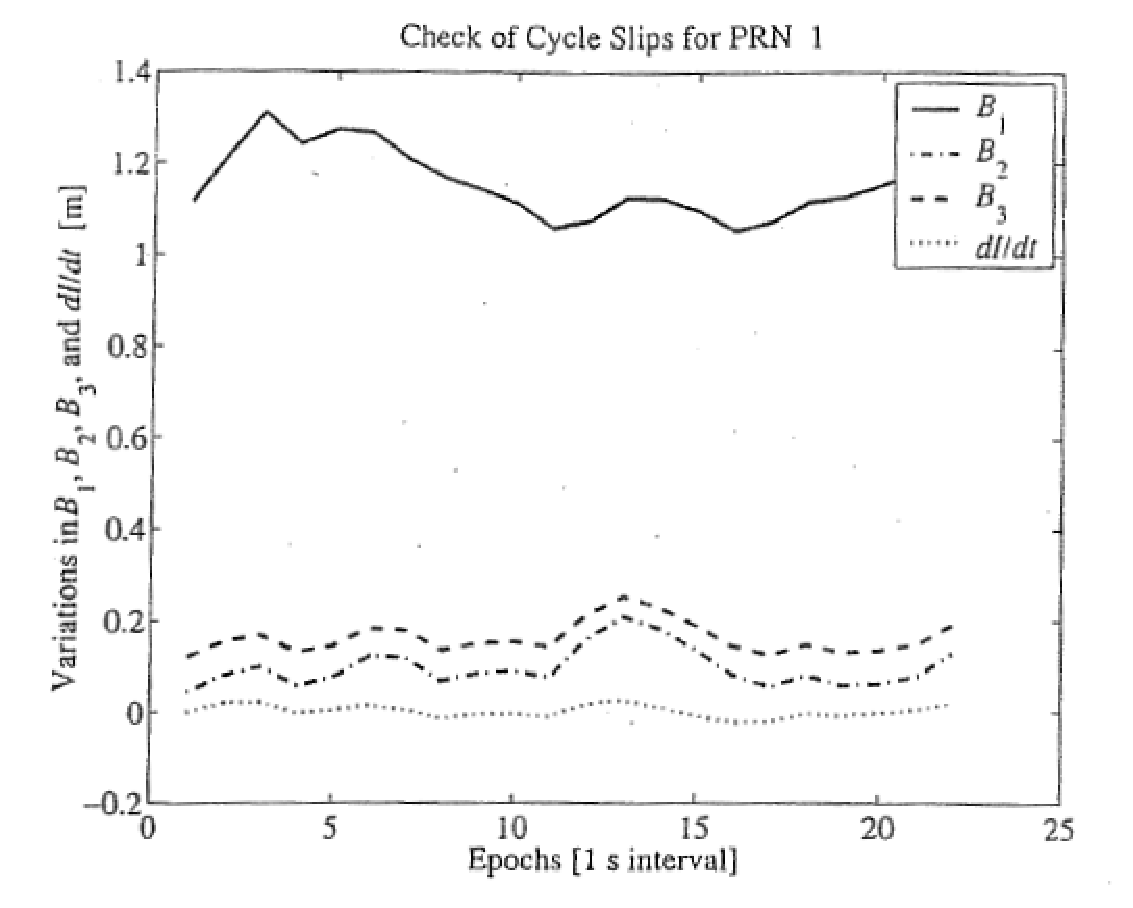
\includegraphics[width=0.4\linewidth]{TeX_files/Part03/chapter10/image/9-3}
	\caption{Check of cycle slips}
	\label{fig:9-3}
\end{figure}

The preliminary data validation can be based on the (single) differences between two receivers. The goal is to detect cycle slips and outliers in the GPS single difference obser
-vations without knowing about satellite and receiver dynamics, their clock behavior and atmospheric effects. It is done independently for each one-way. There is no minimum number of satellites required for this so-called integrity monitoring to work. The following is based on an idea by Kees de Jong (1998).

The dual-frequency single difference measurement model cannot be used directly as it is, since this model is singular. A re-parameterization will make it regular. With hardware delays denoted by $\eta$, the measurement model for epoch k involves the pseudorange R,including hardware delay:$R=\rho+cdt_{i}+T+I+\eta P_{1}$.

\begin{equation}
\begin{bmatrix}
P_{1}\\
P_{2}\\
\Phi_{1}\\
\Phi_{2}\\
\end{bmatrix}
=\begin{bmatrix}
R\\
R\\
R\\
R\\
\end{bmatrix}_{k-1}
+
\begin{bmatrix}
0\\
\eta P_{2}-\eta P_{1}+(\alpha-1)I\\
\eta \Phi_{1}-\eta P_{1}-2I+\lambda_{1}N_{1}\\
\eta \Phi_{2}-\eta P_{1}+(-\alpha-1)I+\lambda_{2}N_{2}\\
\end{bmatrix}_{k-1}
\end{equation}

$P_{1}$ and $P_{2}$ are the pseudorange observables,$\Phi_{1}$ and $\Phi_{2}$ are the carrier phase observables,$N_{1}$ and $N_{2}$ are the carrier phase ambiguities, $\lambda_{1}$ and $\lambda_{2}$ are the wavelengths:$\alpha=(f_{1}/f_{2})^{2}$.

The associated frequencies are $f_{1}$ and $f_{2}$, $\rho$ is the geometric range, and I is the ionospheric delay (all terms are single differenced quantities in units of meters).

R may not change smoothly with time and is hard to model by low-degree polynomials.
But R disappears by subtracting equation 1 from equations 2, 3, and 4:

\begin{equation}
\begin{bmatrix}
P_{2}-P_{1}\\
\Phi_{1}-P_{1}\\
\Phi_{2}-P_{1}\\
\end{bmatrix}_{k}
=\begin{bmatrix}
\alpha-1&0&0\\
0&-2&0\\
0&0&-\alpha-1\\
\end{bmatrix}
\begin{bmatrix}
B_{1}\\
B_{2}\\
B_{3}\\
\end{bmatrix}_{k}
\end{equation}

The covariance matrix includes the �� subtraction matrix�� and its transpose:

$$
\Sigma_{differences}
=
\begin{bmatrix}
-1&1&0&0\\
-1&0&1&0\\
-1&0&0&1\\
\end{bmatrix}
\begin{bmatrix}
\sigma_{P_{1}}^{2}& & & \\
& \sigma_{P_{2}}^{2} & &\\
& &\sigma_{\Phi_{1}}^{2} & \\
& & & \sigma_{\Phi_{2}}^{2} \\
\end{bmatrix}
\begin{bmatrix}
-1&-1&-1\\
1&0&0\\
0&1&0\\
0&0&1\\
\end{bmatrix}_{k}
$$

The parameters $B_{1}$, $B_{2}$ , and $B_{3}$ are linear combinations of the time-dependent ionospheric effect and the constant hardware delays and carrier ambiguities.

The ionospheric effect will be modeled as a first-order polynomial, i.e., as a bias I and a drift $\dot{I}$. The dynamic model (state equation) reads

$$
\begin{bmatrix}
I\\
\dot{I}\\
\end{bmatrix}_{k}
=\begin{bmatrix}
1&t_{k}-t_{k-1}\\
0&1\\
\end{bmatrix}
\begin{bmatrix}
I\\
\dot{I}\\
\end{bmatrix}_{k-1}
$$

In this case $\dot{I}$ = constant. The dynamic model for all parameters then becomes

$$
\begin{bmatrix}
B_{1}\\
B_{2}\\
B_{3}\\
\dot{I}\\
\end{bmatrix}_{k}
=\begin{bmatrix}
1&0&0&t_{k}-t_{k-1}\\
0&1&0&t_{k}-t_{k-1}\\
0&0&1&t_{k}-t_{k-1}\\
0&0&0&1\\
\end{bmatrix}
\begin{bmatrix}
B_{1}\\
B_{2}\\
B_{3}\\
\dot{I}\\
\end{bmatrix}_{k-1}
$$

and the measurement model becomes

$$
\begin{bmatrix}
P_{2}-P_{1}\\
\Phi_{1}-P_{1}\\
\Phi_{2}-P_{1}\\
\end{bmatrix}_{k}
=\begin{bmatrix}
\alpha-1&0&0&0\\
0&-2&0&0\\
0&0&-\alpha-1&0\\
\end{bmatrix}
\begin{bmatrix}
B_{1}\\
B_{2}\\
B_{3}\\
\dot{I}\\
\end{bmatrix}_{k}
$$

With these models and no external information, it is possible to detect a cycle slip in the carrier observations, even when the observation interval $t_{k}-t_{k-1}$ is relatively large.

The actual test for a slip on L2 is $|B_{2,k}-B_{2,k-1}|<\lambda_{1}$, and $|B_{3,k}-B_{3,k-1}|<\lambda_{2}$ on L1. If this test is failed, a cycle slip has occurred and must be repaired.